
\section{Neural networks}

\begin{frame}
	\frametitle{Neurons}

	\centering
        \begin{figure}
                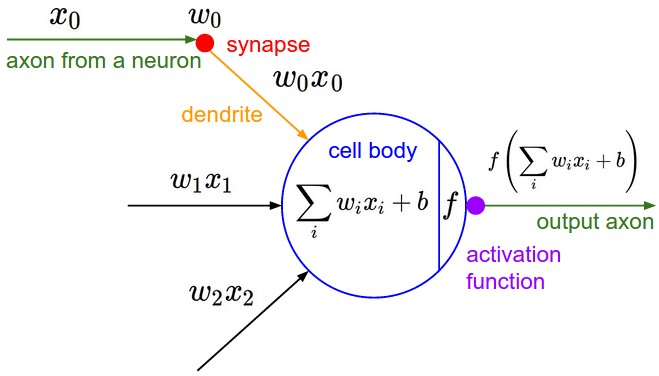
\includegraphics[width=0.7\textwidth]{Pics/neuron_model}
        \end{figure}

\end{frame}

\begin{frame}
	\frametitle{Activation functions}
	
	\centering{It defines the \textit{firing rate}}

	\begin{columns}
		\column{0.5\textwidth}
		\begin{figure}
                	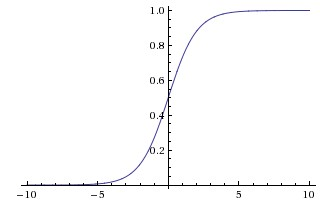
\includegraphics[width=0.7\textwidth]{Pics/sigmoid}\\
			\small{Sigmoid non-linearity squashes real numbers to range between $[0,1]$}
        	\end{figure}
		\column{0.5\textwidth}
		\begin{figure}
                        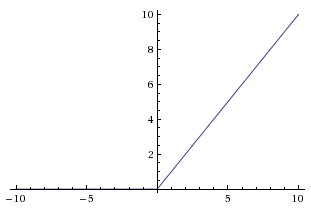
\includegraphics[width=0.7\textwidth]{Pics/relu}\\
                        \small{Rectified Linear Unit (ReLU): $f(x)=max(0,x)$}
                \end{figure}

	\end{columns}

\end{frame}

\begin{frame}
        \frametitle{Neural network architecture}

	Collection of neurons connected in an acyclic graph.\\
	Last output layer represents class scores.

        \begin{columns}
                \column{0.5\textwidth}
                \begin{figure}
                        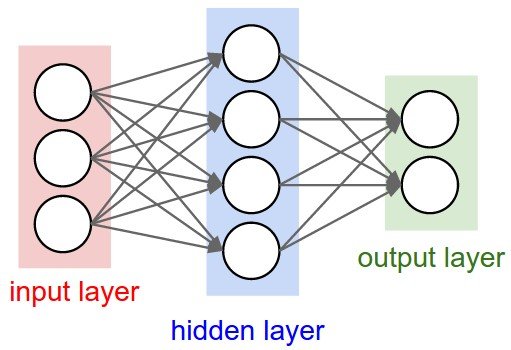
\includegraphics[width=0.7\textwidth]{Pics/neural_net}\\
                        \small{A 2-layer Neural Network}\\
			Size: \pause 4 + 2 = 6 neurons, [3 x 4] + [4 x 2] = 20 weights and 4 + 2 = 6 biases, for a total of 26 learnable parameters.
                \end{figure}
                \column{0.5\textwidth}
                \begin{figure}
                        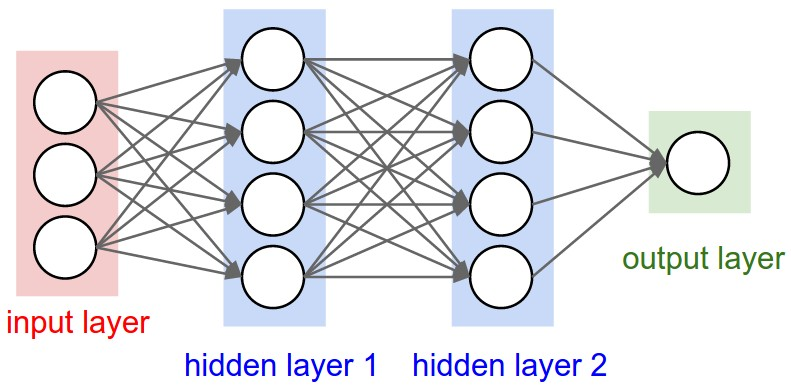
\includegraphics[width=0.7\textwidth]{Pics/neural_net2}\\
                        \small{A 3-layer Neural Network}\\
			Size: \pause 4 + 4 + 1 = 9 neurons, [3 x 4] + [4 x 4] + [4 x 1] = 12 + 16 + 4 = 32 weights and 4 + 4 + 1 = 9 biases, for a total of 41 learnable parameters.
                \end{figure}

        \end{columns}

\end{frame}

\begin{frame}
	\frametitle{Representational power}

	Given any continuous function $f(x)$ and some $\epsilon > 0$, there exists a Neural Network $g(x;W)$ 
	with one hidden layer (with a reasonable choice of non-linearity, e.g. sigmoid) such that for 
	all $x$, $\mid f(x)-g(x) \mid <\epsilon$. 

	\vskip 0.5cm

	In other words, the neural network can approximate any continuous function.

	\vskip 0.5cm

	In practice, more layers work better...

\end{frame}

\begin{frame}
	\frametitle{Setting up the architecture}

	\begin{figure}
        	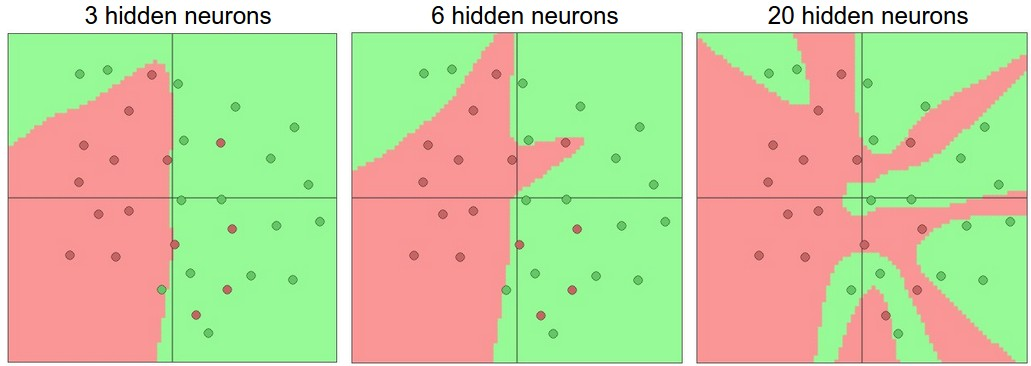
\includegraphics[width=0.8\textwidth]{Pics/layer_sizes}
      	\end{figure}

	Capacity vs. ? \pause Overfitting

	We aim at a better \textbf{generalisation}.

\end{frame}


\begin{frame}
	\frametitle{Setting up the data}

	Data preprocessing:
	\begin{itemize}
		\item mean subtraction
		\item normalisation
		\item PCA and Whitening
	\end{itemize}

\end{frame}


\begin{frame}
        \frametitle{Setting up the model}

        Weights' initialisation:
        \begin{itemize}
                \item all zero
                \item small random numbers
                \item calibrate the variances
		\item sparse
        \end{itemize}

\end{frame}

\begin{frame}
        \frametitle{Setting up the model}

	Regularisation

        \begin{figure}
                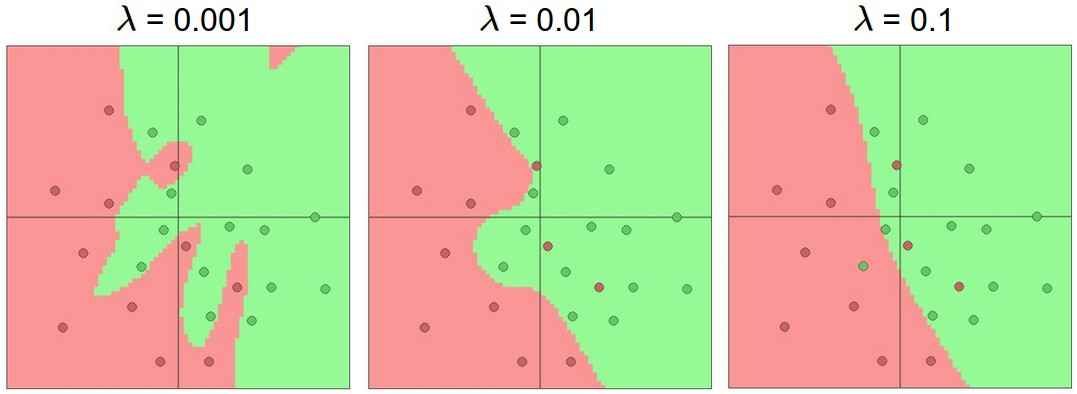
\includegraphics[width=0.8\textwidth]{Pics/reg_strengths}
        \end{figure}

        Options: L2, L1, maxnorm and dropout.

\end{frame}

\begin{frame}
	\frametitle{Dropout}

	\begin{figure}
                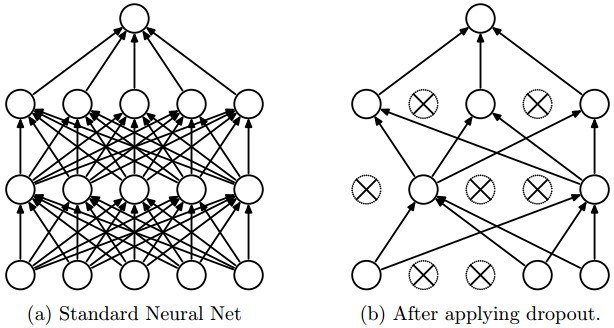
\includegraphics[width=0.8\textwidth]{Pics/dropout}
        \end{figure}

	Dropout can be interpreted as sampling a Neural Network within the full Neural Network, 
	and only updating the parameters of the sampled network based on the input data. 


\end{frame}


\begin{frame}
        \frametitle{Setting up the model}

        Loss functions:
	\begin{itemize}
                \item SVM (hinge loss)
                \item cross-entropy
                \item hierarchical softmax
                \item attribute classification
		\item for regression
        \end{itemize}

\end{frame}

\begin{frame}
	\frametitle{Setting up the learning}

	\begin{columns}
                \column{0.5\textwidth}
                \begin{figure}
                        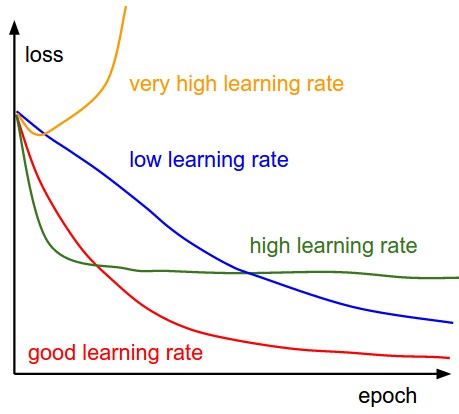
\includegraphics[width=0.8\textwidth]{Pics/learningrates}\\
                        \small{effects of different learning rates}
                \end{figure}
                \column{0.5\textwidth}
                \begin{figure}
                        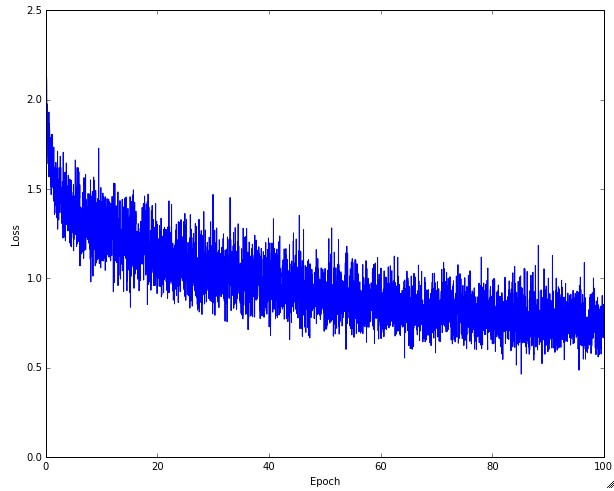
\includegraphics[width=0.8\textwidth]{Pics/loss}\\
                        \small{loss decay}
                \end{figure}

        \end{columns}

\end{frame}

\begin{frame}
        \frametitle{Setting up the learning}

	Training vs. validation accuracy

     	\begin{figure}
     		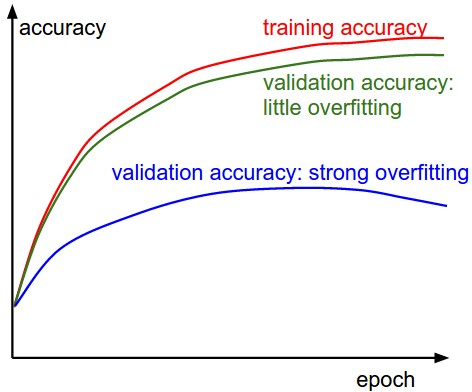
\includegraphics[width=0.5\textwidth]{Pics/accuracies}\\
    	\end{figure}

\end{frame}


\begin{frame}
	\frametitle{Wrap up}

	\begin{itemize}
		\item Neural Networs are made of layers of neurons/units with activation functions
		\item Choice of the architecture: capacity vs overfitting
		\item Preprocessing of the data and choice of hyperparameters for the model and learning
	\end{itemize}

	What about images? Can we use neural networks straight from images? What's the issue?

\end{frame}















